% This is appa.tex
\appendix

\section{An Extended Background}
\label{sec:prelim_background}
Let $V$ be a (real) Euclidean space endowed with a positive definite symmetric bilinear form $(\mu, \lambda)$.
Let $W$ be a group with two generators $s$ and $t$ corresponding to reflecting over two hyperplanes in $V$, and let $\alpha_s$ and $\alpha_t$ be arbitrary vectors normal to these planes.  We assume that the angle formed by $\alpha_s$ and $\alpha_t$ is not a rational multiple of $\pi$, so that the order of $st$ in $W$ is infinite.  

In other words, $W$ is the infinite dihedral group with the presentation \[ W = \left<s,t \mid s^2=t^2=1\right>. \] 

Then for any $a \in V$, reflection over the hyperplane normal to $a$ can be written explicitly for each $v \in V$ as the map \[ v \mapsto v - \frac{2(v,a)}{(a,a)} a. \]  
In particular, if $W$ acts on $V$ by this reflection, $s(\alpha_s) = -\alpha_s$ and $t(\alpha_t) = -\alpha_t$.  Furthermore, using the above, we see that there exist fixed constants $x$ and $y$ such that
\begin{align*}
	s(\alpha_t) &= \alpha_t + x \alpha_s \\
	t(\alpha_s) &= \alpha_s + y \alpha_t
\end{align*}
Explicitly, $x = \frac{-2(\alpha_s,\alpha_t)}{(\alpha_s, \alpha_s)}$ and $y = \frac{-2(\alpha_t,\alpha_s)}{(\alpha_t,\alpha_t)}$.  

Now we define the \emph{Coxeter ring} by $R = \RR[\alpha_s, \alpha_t]$.  Then $W$ acts on $R$ by precisely the same algorithm as described above.

Let $R^s$ be the subring of $R$ which is invariant under $s$.  In other words,
\[ R^s \defeq \left\{ r \in R \mid s(r) = r \right\}. \]
Define $R^t$ similarly.  Then a \emph{Bott-Samelson bimodule} is a bimodule of the form
\[ R \otimes_{R^{i_1}} R \otimes_{R^{i_2}} R \otimes_{R^{i_3}} \dots \otimes_{R^{i_n}} R, \]
where each $i_j$ is either $s$ or $t$.   We write elements of such a bimodule in the form $f_0 \mid f_1 \mid \dots \mid f_n$, where $f_i \in R$.

We consider maps between these bimodules that preserve left and right actions; that is, we consider the maps $\sigma$ such that
\begin{equation}
	\sigma(rx) = r\sigma(x) \quad\text{and}\quad \sigma(xr) = \sigma(x)r \quad\text{for every $r \in R$ and $x \in \text{Domain } \sigma$}.
	\label{eq:respect}
\end{equation}
These maps may be represented diagrammatically.

\subsection{Diagrammatics of Maps}
\label{sec:prelim_map}
\newcommand{\DD}{\mathcal D}
These maps can be described in terms of diagrams.  We take a detour and first describe the appearance of such diagrams; in the subsequent section we will explain their algebraic meaning.  A reader who is not interested in this context can simply accept on faith the relations specified in Appendix~\ref{sec:prelim_genrel}.

Consider a category $\DD$ whose elements are linear combinations $\sum c_i \square$ of the diagrams described below (where the $\square$'s are diagrams).  The coefficients $c_i$ belong to the ring $\ZZ[x,y]$.

The diagrams may be described as planar graphs, not necessarily connected, drawn in a rectangle, with the following properties.
\begin{enumerate}[(i)]
	\ii Vertices may lie on the upper or lower boundary, but not on the left or right boundary.  In other words, the graph is embedded in $\RR \times [0,1]$.
	\ii Each vertex has degree $1$ or $3$.
	\ii Each connected component is colored either blue or red.
\end{enumerate}
The vertices on the boundary are by convention not explicitly shown, but are nonetheless labelled $s$ or $t$ for blue or red, respectively.

\begin{figure}[ht]
	\centering
	\begin{asy}
	size(6cm);
	real xmax=7;
	real ymax=5;
	draw( (xmax,ymax)--(xmax,-ymax)--(-xmax,-ymax)--(-xmax,ymax)--cycle );
	pair apex = (0,2);
	path arc = (5,-5)..(2,0)..apex..(-2,0)..(-5,-5);
	draw(arc, s);
	dot(apex, dot_s);
	draw(apex--(0,ymax), s);
	draw(-apex--(0,-ymax), t);
	dot(-apex, dot_t);
	label("$s$", (0,ymax), dir(90));
	label("$t$", (0,-ymax), dir(270));
	label("$s$", (-5,-ymax), dir(270));
	label("$s$", (5,-ymax), dir(270));
	\end{asy}
	\caption{An example of a possible diagram.}
	\label{fig:example_diagram}
\end{figure}

An example of such a diagram is shown in Figure~\ref{fig:example_diagram}.

The elements of $\DD$ can be added by simply adding corresponding coefficients in front of each diagram; no other relations exist.  Multiplication is defined as follows: the product of two diagrams is the composition of the diagrams if the labels on the bottom of the first coincide with those on the top of the second.  By composition, we mean that the first diagram is vertically juxtaposed on top of the second diagram; see Figure~\ref{fig:example_compose} for an example.  Otherwise, the product is $0$.

\subsection{Algebraic Context}
\label{sec:prelim_alg_context}
The maps are conventionally read from bottom to top.  The labels on the upper and lower boundaries specify the domain and codomain of the map by ``transcribing'' the tensor products to take -- for example, a map with bottom $stt$ and top $s$ represents a map with domain $R \stimes R \ttimes R \ttimes R$ and codomain $R \stimes R$.  An unlabelled domain corresponds to $R$.

Let us introduce one final definition.
\begin{definition}
	The \emph{Demazure operator} $\partial_s: R \to R$ is given by \[ \partial_s(f) = \frac{f - s(f)}{\alpha_s}. \]
\end{definition}

With this, we can now describe the meanings of each type of vertex (for blue lines) in Table~\ref{tab:prim_maps}.  The corresponding equations hold for red in $t$.

\begin{table}[ht]
	\[
	\begin{array}{rll}
		\text{Map} & \text{Modules} & \text{Description} \\[1em]
		\barbell{
\includegraphics{barbell/half_top.pdf}} & R \stimes R \to R & 1 \mid 1 \mapsto 1 \\[1em]
		\barbell{
\includegraphics{barbell/half_bot.pdf}} & R \to R \stimes R & 1 \mapsto \half \left( 1 \mid \alpha_s + \alpha_s \mid 1 \right) \\[1em]
		\barbell{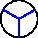
\includegraphics{barbell/tri_down.pdf}} & R \stimes R \to R \stimes R \stimes R & 1 \mid 1 \mapsto 1 \mid 1 \mid 1 \\[1em]
		\barbell{
\includegraphics{barbell/tri_up.pdf}} & R \stimes R \stimes R \to R \stimes R & 1 \mid g \mid 1 \mapsto \partial_s(g) \mid 1 \\[1em]
		\barbell{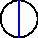
\includegraphics{barbell/id.pdf}} & R \stimes R \to R \stimes R & 1 \mid 1 \mapsto 1 \mid 1 \\[1em]
	\end{array}
	\]
	\caption{Describing the maps.}
	\label{tab:prim_maps}
\end{table}

Note that the descriptions are sufficient to determine outputs for all values because these morphisms respect left and right actions, as prescribed in \eqref{eq:respect}.

Maps are composed by juxtaposition, and disjoint portions of the diagrams act independently.  Therefore, by a combination of these structures, we can generate arbitrarily complicated maps.  
\begin{example*}
	The diagram in Figure~\ref{fig:example_diagram} represents a map \[ R \stimes R \ttimes R \stimes R \to R \stimes R \quad\text{by}\quad a \mid b \mid c \mid d \mapsto a \partial_s(bc) \mid d. \]
\end{example*}

Henceforth, we will make the convenient abbreviation of $\barbell{
\includegraphics{barbell/tri_up_contract_before.pdf}}$ as $\barbell{
\includegraphics{barbell/tri_up_contract_after.pdf}}$.  It will also be understood that edges need not be straight lines, but any topologically equivalent deformation shall represent the same graph.  With this understanding, any of the graphs described in the previous section can be viewed as compositions of the primitive structures we describe here.

\subsection{Operations for Diagrammatics}
\label{sec:prelim_genrel}
From the algebraic context given above, one can derive the following relationships, which are here described completely graphically.  These rules are sufficient to compute the maps we are interested in.  

Unless multiple colors appear in an equation, blue represents a generic color.

\setcounter{op}{-1}
\begin{op}[Isotropy] If two diagrams can be continuously deformed into each other (in the topological sense), then they are equivalent.  In other words, the maps are isotropy invariant  \end{op}
\begin{remark*}
	The justification for the above operation is not obvious; see page 7 of \cite{ref:gr4all} for an explanation.
\end{remark*}
\begin{op}[Associativity] We have $\barbell{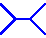
\includegraphics{barbell/assoc_horiz.pdf}} = \barbell{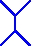
\includegraphics{barbell/assoc_vert.pdf}}$.  \end{op}
\begin{op}[Contraction] We have $\barbell{
\includegraphics{barbell/contract_left.pdf}} = \barbell{
\includegraphics{barbell/contract_right.pdf}} = \barbell{
\includegraphics{barbell/alpha_blue.pdf}}$.  \end{op}
\begin{op}[The Needle] We have $\barbell{
\includegraphics{barbell/needle.pdf}} = 0$.  \end{op}
\begin{remark*} Using contraction and the above, one can show that the diagram $\barbell{
\includegraphics{barbell/zero.pdf}}$ is zero as well. In fact, in general, \emph{any} map which contains a ``closed'' and empty region is the zero map.  \end{remark*}
\begin{op}[Barbell-Forcing Rules]
	We have the following three equalities:
	\begin{enumerate}[(a)]
		\ii $\barbell{
\includegraphics{barbell/barbell_blue.pdf}}\barbell{
\includegraphics{barbell/alpha_blue.pdf}} + \barbell{
\includegraphics{barbell/alpha_blue.pdf}} \barbell{
\includegraphics{barbell/barbell_blue.pdf}} = 2 \barbell{
\includegraphics{barbell/break_blue.pdf}}$, and the similar equation for red.
		\ii $\barbell{
\includegraphics{barbell/alpha_red.pdf}}\barbell{
\includegraphics{barbell/barbell_blue.pdf}} = -x\barbell{
\includegraphics{barbell/break_red.pdf}} + \barbell{
\includegraphics{barbell/barbell_blue.pdf}}\barbell{
\includegraphics{barbell/alpha_red.pdf}} + x \barbell{
\includegraphics{barbell/barbell_red.pdf}}\barbell{
\includegraphics{barbell/alpha_red.pdf}}$.
		\ii $\barbell{
\includegraphics{barbell/alpha_blue.pdf}}\barbell{
\includegraphics{barbell/barbell_red.pdf}} = -y\barbell{
\includegraphics{barbell/break_blue.pdf}} + \barbell{
\includegraphics{barbell/barbell_red.pdf}}\barbell{
\includegraphics{barbell/alpha_blue.pdf}} + y \barbell{
\includegraphics{barbell/barbell_blue.pdf}}\barbell{
\includegraphics{barbell/alpha_blue.pdf}}$.
	\end{enumerate}
\end{op}

\subsection{Libedinsky's Light Leaves}
\label{sec:prelim_lightleave}
\begin{figure}[ht]
	\centering
	\begin{asy}
	size(10cm);
	real h = 0.7;
	draw(currentpicture, (0,0)--(0,h/2)..((0+2)/2.0,h*2)..(2,h/2)--(2,0), s);
	draw(currentpicture, (2,0)--(2,h/2)..((2+3)/2.0,h*1)..(3,h/2)--(3,0), s);
	draw(currentpicture, (5,0)--(5,h/2)..((5+6)/2.0,h*1)..(6,h/2)--(6,0), s);
	draw(currentpicture, (4,0)--(4,h/2)..((4+8)/2.0,h*4)..(8,h/2)--(8,0), t);
	draw(currentpicture, (8,0)--(8,h/2)..((8+9)/2.0,h*1)..(9,h/2)--(9,0), t);
	draw(currentpicture, (11,0)--(11,h/2)..((11+13)/2.0,h*2)..(13,h/2)--(13,0), t);
	draw(currentpicture, (1,0)--(1,h), t);dot(currentpicture, (1,h), red);
	draw(currentpicture, (7,0)--(7,h), s);dot(currentpicture, (7,h), s);
	draw(currentpicture, (12,0)--(12,h), s);dot(currentpicture, (12,h), s);
	draw(currentpicture,(9,0)--(9,5*h), t);
	draw(currentpicture,(10,0)--(10,5*h), s);
	dot(currentpicture, (2, h/2), blue);
	dot(currentpicture, (8, h/2), red);
	dot(currentpicture, (9, h/2), red);
	label(currentpicture, "1", (0,-1.5h), dir(90));
	label(currentpicture, "s", (0,-0.8*h), dir(90));
	label(currentpicture, "0", (1,-1.5h), dir(90));
	label(currentpicture, "t", (1,-0.8*h), dir(90));
	label(currentpicture, "0", (2,-1.5h), dir(90));
	label(currentpicture, "s", (2,-0.8*h), dir(90));
	label(currentpicture, "1", (3,-1.5h), dir(90));
	label(currentpicture, "s", (3,-0.8*h), dir(90));
	label(currentpicture, "1", (4,-1.5h), dir(90));
	label(currentpicture, "t", (4,-0.8*h), dir(90));
	label(currentpicture, "1", (5,-1.5h), dir(90));
	label(currentpicture, "s", (5,-0.8*h), dir(90));
	label(currentpicture, "1", (6,-1.5h), dir(90));
	label(currentpicture, "s", (6,-0.8*h), dir(90));
	label(currentpicture, "0", (7,-1.5h), dir(90));
	label(currentpicture, "s", (7,-0.8*h), dir(90));
	label(currentpicture, "0", (8,-1.5h), dir(90));
	label(currentpicture, "t", (8,-0.8*h), dir(90));
	label(currentpicture, "0", (9,-1.5h), dir(90));
	label(currentpicture, "t", (9,-0.8*h), dir(90));
	label(currentpicture, "1", (10,-1.5h), dir(90));
	label(currentpicture, "s", (10,-0.8*h), dir(90));
	label(currentpicture, "1", (11,-1.5h), dir(90));
	label(currentpicture, "t", (11,-0.8*h), dir(90));
	label(currentpicture, "0", (12,-1.5h), dir(90));
	label(currentpicture, "s", (12,-0.8*h), dir(90));
	label(currentpicture, "1", (13,-1.5h), dir(90));
	label(currentpicture, "t", (13,-0.8*h), dir(90));
	\end{asy}
	\caption{An example of a light leaf.}
	\label{fig:lightleaf_example}
\end{figure}
We now present the algorithm for Libedinsky's light leaves, in the special case where $W$ is the infinite dihedral group.  A full construction for more general Coxeter groups is given in \cite{ref:gr4all}.

Fix an expression $\ul r$ of length $n$.  Then for any binary string $\ul b$ of length $n$ we can construct a diagram based on a series of rules.

Each bit of $\ul b$ is read from left to right in order and designated either open or closed; the state of a bit can change more than once.  Initially all bits are closed.  We say that a bit $x$ is an \emph{open neighbor} of $y$ if $x$ is marked open, $x$ and $y$ have the same color, and there are no other bits marked open between $x$ and $y$.  Note that each bit will have at most one open neighbor.

\begin{itemize}
	\ii If the bit is a $1$:
	\begin{itemize}
		\ii If the current bit has an open neighbor, then draw an arc joining the two bits, and mark both bits as closed.
		\ii Otherwise, designate the current bit as open.
	\end{itemize}
	\ii If the bit is $0$:
	\begin{itemize}
		\ii If the current bit has an open neighbor, then draw an arc joining the two bits, mark the previous bit as closed, and the current bit as open.
		\ii Otherwise, create a ``stub'', i.e. a single vertex of degree one, and mark the current bit as down.
	\end{itemize}
\end{itemize}
Finally, join any bits which are open at the end of the process to the upper boundary of the diagram.  A map which arises in such a manner is called a \emph{light leaf}.  An example of such a light leaf is shown in Figure~\ref{fig:lightleaf_example}.

The \emph{top} of such a map is the expression which appears on the upper boundary; i.e. the bits which are still up at the end of the algorithm.  For example, the map in Figure~\ref{fig:lightleaf_example} has top $ts$.  Note that any top is a reduced expression.  


\section{Proof of the One-Color Theorem}
\label{sec:s_proof}
\begin{figure}[ht]
	\centering
	\begin{asy}
		size(7cm);
		real h = 0.7;
		int n = 8;
		draw(currentpicture, (0,0)--(0,h/2)..((0+1)/2.0,h*1)..(1,h/2)--(1,0), s);
		draw(currentpicture, (1,0)--(1,h/2)..((1+2)/2.0,h*1)..(2,h/2)--(2,0), s);
		draw(currentpicture, (2,0)--(2,h/2)..((2+3)/2.0,h*1)..(3,h/2)--(3,0), s);
		draw(currentpicture, (5,0)--(5,h/2)..((5+6)/2.0,h*1)..(6,h/2)--(6,0), s);
		draw(currentpicture, (4,0)--(4,h), s);
		dot(currentpicture, (4,h), dot_s);
		draw(currentpicture, (7,0)--(7,h), s);
		dot(currentpicture, (7,h), dot_s);
		dot(currentpicture, (1, h/2), dot_s);
		dot(currentpicture, (2, h/2), dot_s);
		label(currentpicture, "1", (0,-1.5h), dir(90));
		label(currentpicture, "s", (0,-0.8*h), dir(90));
		label(currentpicture, "0", (1,-1.5h), dir(90));
		label(currentpicture, "s", (1,-0.8*h), dir(90));
		label(currentpicture, "0", (2,-1.5h), dir(90));
		label(currentpicture, "s", (2,-0.8*h), dir(90));
		label(currentpicture, "1", (3,-1.5h), dir(90));
		label(currentpicture, "s", (3,-0.8*h), dir(90));
		label(currentpicture, "0", (4,-1.5h), dir(90));
		label(currentpicture, "s", (4,-0.8*h), dir(90));
		label(currentpicture, "1", (5,-1.5h), dir(90));
		label(currentpicture, "s", (5,-0.8*h), dir(90));
		label(currentpicture, "1", (6,-1.5h), dir(90));
		label(currentpicture, "s", (6,-0.8*h), dir(90));
		label(currentpicture, "0", (7,-1.5h), dir(90));
		label(currentpicture, "s", (7,-0.8*h), dir(90));
	\end{asy}
	\caption{A half-map with base $\SS_8$.}
	\label{fig:pf_trivial_theorem_example}
\end{figure}

\onecolor*
\begin{proof}[Proof of Theorem \ref{thm:onecolor}]
	We will only consider the case where $\Top(\ul a) = \varnothing$, so that $\ul a^\ast[n] = \ul b^\ast[n] = 0$; the other case is essentially identical.  See Figure~\ref{fig:pf_trivial_theorem_example} for a example of such a map.

	Number the anchors $1,2,\dots,n$ from left to right.  For a half-map $\MM(\ul b)$, define the \emph{antennae} of a connected component to be the anchors which it touches.  Note that the antennae of a component always form a single contiguous sequence of anchors.

	The key observation is that for $1 \le i \le n-1$, we have that $\ul b^\ast[i] = 1$ if and only if $i$ and $i+1$ are both antennae of some component in $\MM(\ul b)$.  This follows by construction.

	Let us now compose $M_a \defeq \MM(\ul a)$ and $M_b \defeq \MM(\ul b)$ to obtain a full-map.  Two components (one from $M_a$ and one from $M_b$) are said to \emph{feel} each other $k$ times if they have $k$ antennae in common.  Notice that if any two components feel each other at least twice, then there exist two adjacent common antennae, forcing the composition of the entire map to be zero because the two antennae combine to form an empty bubble.  Furthermore, it is evident that any bubbles must be formed in this manner.  In combination with the claim above, this implies the first case of the theorem.

	On the other hand, suppose this product is nonzero, and consider a component from the top with $k$ antennae.  It suffices to show that there are $n - \pi_1(\ul a^\ast) - \pi_1(\ul b^\ast)$ barbells.  Notice that $\pi_1(\ul a^\ast) + \pi_1(\ul b^\ast)$ counts the number of edges between adjacent anchors ($i$ and $i+1$).  Because there are no cycles, deleting one of these edges increases the number of connected components by exactly one (since all the connected components are barbells).  If we delete all such edges, then we obtain $n$ barbells.  Therefore there must have been $n - \pi_1(\ul a^\ast) - \pi_1(\ul b^\ast)$ barbells to begin with, as desired.
\end{proof}

\section{Computation for Map Counting}
\label{sec:count_map_computation}
\defredcountmaps*
\countmaps*
The main idea of the proof was given earlier on page~\pageref{thm:count_maps}.  Here are the details.

\begin{proof}[Proof of Proposition \ref{thm:count_maps}]
	First we resolve the case where $\ul r = \AA_n$, so that $\ell = n$ and $2^{\ell-n} = 1$.  We proceed by induction on $n \ge 1$ and consider eight cases.  (The base case is trivial.) The strategy for each is that, for the binary strings of length $n$ and top $\ul w$, we consider those binary strings which end with $1$ and those which end with $0$.  Using \eqref{eq:top}, we may then write the new quantity in terms of the number of strings of length $n-1$ with a different top.

	When $n = 2k+1$, we have $\AA_n[n] = s$ and $n-1 = 2k$.  Let $\ul b'$ denote the first $n-1$ characters of $\ul b$.  Then,
	\newcommand{\aoeu}[5]{The top #1 ends in #2.  So, if $\ul b[n] = 1$ then we have top #3 for $\ul b'$, and otherwise $\ul b'$ has the same top #4.  In total, we get #5.}
	\begin{itemize}
		\ii \aoeu{$\AA_{2m+1}$}{$s$}{$\AA_{2m} = \AA_{2(m-1)+2}$}{$\AA_{2m+1}$}%
		{$\binom{n-2}{(m-1)+k} + \binom{n-2}{m+k} = \binom{n-1}{m+k}$}
		\ii \aoeu{$\AA_{2m}$}{$t$}{$\AA_{2m+1}$}{$\AA_{2m} = \AA_{2(m-1)+2}$}%
		{$\binom{n-2}{m+k} + \binom{n-2}{(m-1)+k} = \binom{n-1}{m+k}$}
		\ii \aoeu{$\AA_{2m-1}'$}{$t$}{$\AA_{2m}'$}{$\AA_{2m-1}' = \AA_{2(m-1)+1}'$}%
		{$\binom{n-2}{m+k} + \binom{n-2}{(m-1)+k} = \binom{n-1}{m+k}$}
		\ii \aoeu{$\AA_{2m}'$}{$s$}{$\AA_{2m-1}' = \AA_{2(m-1)+1}'$}{$\AA_{2m}'$}%
		{$\binom{n-2}{(m-1)+k} + \binom{n-2}{m+k} = \binom{n-1}{m+k}$}
	\end{itemize}
	The case where $n=2k$ is similar, but we now have $n-1=2(k-1)+1$.  Now the last bit changes the top by $t$.
	\begin{itemize}
		\ii \aoeu{$\AA_{2m+1}$}{$s$}{$\AA_{2m+2} = \AA_{2(m+1)}$}{$\AA_{2m+1}$}%
		{$\binom{n-2}{(m+1)+(k-1)} + \binom{n-2}{m+(k-1)} = \binom{n-1}{m+k}$}
		\ii \aoeu{$\AA_{2m+2}$}{$t$}{$\AA_{2m+1}$}{$\AA_{2m+2} = \AA_{2(m+1)}$}%
		{$\binom{n-2}{m+(k-1)} + \binom{n-2}{(m+1)+(k-1)} = \binom{n-1}{m+k}$}
		\ii \aoeu{$\AA_{2m}'$}{$s$}{$\AA_{2m+1}' = \AA_{2(m+1)-1}'$}{$\AA_{2m}'$}%
		{$\binom{n-2}{(m+1)+(k-1)} + \binom{n-2}{m+(k-1)} = \binom{n-1}{m+k}$}
		\ii \aoeu{$\AA_{2m+1}'$}{$t$}{$\AA_{2m}'$}{$\AA_{2m+1}'=\AA_{2(m+1)-1}'$}%
		{$\binom{n-2}{m+(k-1)} + \binom{n-2}{(m+1)+(k-1)} = \binom{n-1}{m+k}$}
	\end{itemize}
	This completes the inductive step.  Hence, the proposition is true for $\ell = n$.

	To finish the case $\ell \neq n$, we note that we can treat each consecutive block of $s$'s of length $m$ as a single $s$, where there are $2^{m-1}$ ways to get a $1$ and $2^{m-1}$ ways to get a $0$.  (This follows from Proposition~\ref{prop:s_top}.)  This reduces to the previous case $\ul r = \AA_n$ multiplied by additional factors of $2$; aggregating all of them yields the factor of $2^{\ell-n}$, as desired.
\end{proof}



\section{Proofs of Lemmata}
\label{sec:lemmata_proof}
\subsection{Proof of the Bubble Lemma}
We begin with a proof of the Bubble Lemma\footnote{I should remark that attempting to construct counterexamples to the Bubble Lemma leads to a far better understanding than trying to read the following proof.}, which is the fundamental lemma for the alternating case.  Indeed, both of the subsequent lemmas are fairly straightforward consequences of this one.  

\bubble*
\begin{proof}[Proof of Lemma \ref{thm:bubble}]
	Take a bubble $B$ and assume without loss of generality that it is blue.  By construction all caterpillars held inside $B$ must be red.  This implies that there must be at least one red caterpillar, because there is at least one red anchor inside $B$.

	Define a pair of red anchors $u, v$, with $u$ to the left of $v$, to be \emph{quasi-connected} if
	\begin{inparaenum}[(i)]
		\ii one can draw an arc from $u$ to $v$ contained entirely in one half-map which does not intersect blue lines, and
		\ii there is no red anchor $w$ strictly between $u$ and $v$ for which one can draw a similar arc on the same half-map joining $w$ and $v$.
	\end{inparaenum}

	Now we claim that \textbf{any quasi-connected pair of red anchors is actually joined by a red arc}.  To prove this, take such a quasi-connected pair $u$ and $v$.  Now we'll focus only on the half-map in which the prescribed arc is drawn.  We thus may state that an arc \emph{shields} any anchors which lie between its endpoints.
	
	\begin{figure}[ht]
		\centering
		\begin{asy}
			size(6cm);
			for (int i=0; i<=8; i+=2) { dot( (i,0), dot_s ); }
			for (int i=1; i<=8; i+=2) { dot( (i,0), dot_t ); }
			draw((0,0)..(1,2)..(3,4)..(5,3)..(6,5)..(7,2)..(8,0), s);
			draw((1,0)..(3,2)..(5,0), t); // red covering arc
			draw((2,0)..(3,1)..(4,0), s); // blue covering arc again
			label("$A$", (4.1,1.6), dir(60));
			label("$u$", (3,0), dir(-90));
			label("$x$", (4,0), dir(-90));
			label("$v$", (5,0), dir(-90));
		\end{asy}
		\hspace{2em}
		\begin{asy}
			size(6cm);
			for (int i=0; i<=8; i+=2) { dot( (i,0), dot_s ); }
			for (int i=1; i<=8; i+=2) { dot( (i,0), dot_t ); }
			draw((0,0)..(1,2)..(3,4)..(5,3)..(6,5)..(7,2)..(8,0), s);
			draw((1,0)..(4,2)..(7,0), t); // red covering arc
			draw((2,0)..(4,1)..(6,0), s); // blue covering arc
			label("$A$", (5.6,1.5), dir(60));
			label("$u$", (3,0), dir(-90));
			label("$x$", (4,0), dir(-90));
			label("$v$", (5,0), dir(-90));
		\end{asy}
		\caption{Proving the bubble lemma with quasi-connected vertices.}
		\label{fig:pf_bubble}
	\end{figure}
	Because the string is alternating, we can take a blue anchor $x$ immediately to the left of $v$.  Now, there must be some blue arc shielding $u$ and $v$ (since $u,v$ are inside a blue bubble).  By construction, there must be some red arc $A$ covering $x$.  If this arc joins $u$ and $v$, then we are done.  
	Otherwise, if it has endpoint $v$ then it must completely cover $u$ by condition (ii) of quasi-connectedness; if not, then it must completely cover $v$.  This leads us to two cases.
	\begin{itemize}
		\ii If the arc covers exactly one of $u$ or $v$, say $u$, then there must be a blue arc shielding $u$ from $A$.  But then this contradicts the quasi-connectedness, because now it is not possible to join $u$ and $v$ by an arc on this half-map.  This case is illustrated by the left half of Figure~\ref{fig:pf_bubble}.
		\ii If the arc covers both $u$ and $v$, then there must be a blue arc which shields both $u$ and $v$, which is itself shielded by $A$.  Then we can repeat the same procedure with this new blue arc.  This case is illustrated by the right half of Figure~\ref{fig:pf_bubble}.
	\end{itemize}
	Therefore any pair of quasi-connected anchors must be connected by an arc.  However, one can verify that the red anchors in $B$ but not in any other bubble are ``connected'' under quasi-connectedness.\footnote{That is, one can follow a sequence of red anchors, each consecutive pair quasi-connected, from any red anchor to any other red anchor.}  Therefore all such red anchors must be connected.  So there is a single caterpillar, as desired.
\end{proof}

\subsection{Proof of the Caterpillar Lemma}
We will now derive the Caterpillar Lemma as a consequence of the Bubble Lemma.  
\caterpillar*

It is worth intuitively explaining the main idea of the proof; the rest is book-keeping.  Essentially, because caterpillars may only hold a single other caterpillar, we may ``descend down'' until we find a caterpillar which contains barbells in its bubbles.  Now we break each of the bubbles of this caterpillar one at a time using the barbell forcing rule.  This generates several $x$ and $y$ terms, but the barbell disappears at each such move.  Hence, we break all cycles in the caterpillar, at which point it becomes a barbell (modulo the addition of new $x$ and $y$ terms).  Rinse and repeat.

First, a few definitions for this section only.
\begin{definition}
	Consider a caterpillar $C$ in a full-diagram with base $\AA_n$.  Define the \emph{nesting level} of the caterpillar as the largest integer $n$ for which there exists caterpillars $C = C_0$, $C_1$, $C_2$, $\dots$, $C_n$ such that $C_i$ holds $C_{i+1}$ for each $i=0,1,\dots,n-1$.  Define the \emph{size} of the caterpillar to be the number of bubbles it contains.
\end{definition}

\begin{proof}[Proof of Lemma \ref{thm:caterpillar}]
	The proof is by double induction.  First we will consider caterpillars with nesting level $0$.  

	We perform induction on the size of the caterpillar. 
	If there are no bubbles, then the caterpillar is simply a barbell.
	This is the base step.
	For the inductive step, consider an arbitrary bubble.  Inside it is exactly one caterpillar, say $c$, by the Bubble Lemma.  Because the original caterpillar has nesting level $0$, we deduce $c$ is merely a barbell, and hence is either $\alpha_s$ or $\alpha_t$.
	Applying the barbell-forcing rule of equation \eqref{eq:barbell_break} generates two terms.  One of them is zero because it creates a new empty bubble. The other is the original diagram with the cycle cut open and the contents removed, multiplied by one of $\left\{ x,y \right\}$.  The inductive hypothesis now applies directly, and this completes the first induction.

	Now suppose a caterpillar has nesting level $k \ge 1$.  We simply apply the exact same induction on size as before.  The only modification is that, instead of a barbell, we have a caterpillar with nesting level strictly less than $k$.  However, these caterpillars all evaluate as a polynomial again of the form $x^my^n \alpha_s$ or $x^my^n\alpha_t$, by the outer inductive hypothesis.  So applying equation \eqref{eq:barbell_break} in the same manner completes this induction as well.
\end{proof}

\subsection{Proof of the Pasture Lemma}
\begin{figure}[ht]
	\centering
	\begin{asy}
		size(11cm);
		real h = 0.7;
		int n = 6;

		picture before;
		draw(before, (1,0)--(1,h/2)..((1+3)/2.0,h*2)..(3,h/2)--(3,0), t);
		draw(before, (2,0)--(2,h), s);
		dot(before, (2,h), dot_s);
		draw(before, (5,0)--(5,h), t);
		dot(before, (5,h), dot_t);
		draw(before,(0,0)--(0,3*h), s);
		draw(before,(3,0)--(3,3*h), t);
		draw(before,(4,0)--(4,3*h), s);
		dot(before, (3, h/2), dot_t);

		add(before); add(reflect((0,0),(1,0))*before);
		draw((-1,0)--(6,0));

		picture after;
		draw(after, (1,0)--(1,h/2)..((1+3)/2.0,h*2)..(3,h/2)--(3,0), t);
		draw(after, (4,0)--(4,h/2)..((4+6)/2.0,h*2)..(6,h/2)--(6,0), s);
		draw(after, (3,0)--(3,h/2)..((3+7)/2.0,h*4)..(7,h/2)--(7,0), t);
		draw(after, (0,0)--(0,h/2)..((0+8)/2.0,h*5.5)..(8,h/2)--(8,0), s);
		draw(after, (2,0)--(2,h), s);
		dot(after, (2,h), dot_s);
		draw(after, (5,0)--(5,h), t);
		dot(after, (5,h), dot_t);
		dot(after, (3, h/2), dot_t);

		add(shift((9,0)) * after);
		add(shift((9,0)) * reflect((0,0),(1,0))*after);
		draw((8,0)--(18,0));

		label("$\to$", (7,0));
	\end{asy}
	\caption{In the first diagram, $\ul a = \ul b = 110010$.  In the second, $\ul a' = \ul b' = 110010111$.  Closing the pastures allows us to deduce the Pasture Lemma from the Bubble Lemma.}
	\label{fig:pf_pasture}
\end{figure}
The Bubble Lemma and the Pasture Lemma are structurally very similar.  In fact, we will now show a somewhat surprising proof that the Pasture Lemma follows from the Bubble Lemma.

\pasture*
\begin{proof}[Proof of Lemma \ref{thm:pasture}]
	Again, let $\ul w$ denote the top, with length $N$.  In the first case, suppose $\ul w[N] \neq \AA_n[n]$; that is, the last characters of $\ul w$ and $\AA_n$ differ.  Then it must be the case that the rightmost anchor is not part of a fence.
	Now suppose the map arose from $\MM_{\AA_n}(\ul a, \ul b)$.  Let $\ul a'$ be the string formed by appending $N$ $1$'s to $\ul a$, and define $\ul b'$ similarly.  Now consider the map \[ \MM_{\AA_{n+N}} \left( \ul a', \ul b' \right). \]  See Figure~\ref{fig:pf_pasture} for an example.

	Clearly the top of this new map is zero, say by \eqref{eq:top}.  Now what we have done is enclose the contents of each pasture into bubbles.  The Bubble Lemma tells us that the innermost bubble can have exactly one caterpillar, while the other bubbles must contain only a single caterpillar, which was once a fence.  This implies the Pasture Lemma in the first case.

	The case where $\ul w[N] = \AA_n[n]$ is similar.  We simply append a zero followed by $N$ $1$'s and repeat the same procedure.  The only difference is that the innermost barbell was generated by the $0$ we appended, and thus was not part of the original diagram.
\end{proof}



\section{Proof of the Alternating Recursion}
\label{sec:recurse_proof}
\recurse*
\begin{proof}[Proof of Proposition \ref{thm:recurse}]
	We will only resolve the case where $n$ is odd; that is, $\AA_n$ terminates in $s$.  The other case is identical.
	\begin{enumerate}[(i)]
		\ii Suppose $\ul a[n] = \ul b[n] = 0$.  Note that the top of $M_1$ is also $\ul w$.
		\begin{itemize}
			\ii If $\ul w = \varnothing$, then $M_1$ also had top $\varnothing$.  Therefore, the addition of the $0$'s at the end simply generates an extra blue barbell.  So the resulting map is simply a multiple by $\alpha_s$; i.e. $M = \alpha_sM_1$.
			\ii The case where $\ul w$ ends in $t$ is analogous; we simply obtain a new barbell.  However, because $\ul w \neq \varnothing$, the extra factor is $Q_{\ul w}$ instead of simply $\alpha_t$.  Hence, $M = Q_{\ul w}M_1$.
			\begin{figure}[ht]
				\centering
				\begin{asy}
					size(12cm);
					real h = 0.7;
					int n = 4;

					picture one;
					draw(one, (0,0)--(0,h/2)..((0+2)/2.0,h*2)..(2,h/2)--(2,0), s);
					draw(one, (1,0)--(1,h), t);
					dot(one, (1,h), dot_t);
					draw(one, (3,0)--(3,h), t);
					dot(one, (3,h), dot_t);
					draw(one,(2,0)--(2,3*h), s);
					dot(one, (2, h/2), dot_s);

					picture two;
					draw(two, (0,0)--(0,h), s);
					dot(two, (0,h), dot_s);
					draw(two, (1,0)--(1,h), t);
					dot(two, (1,h), dot_t);
					draw(two, (3,0)--(3,h), t);
					dot(two, (3,h), dot_t);
					draw(two,(2,0)--(2,3*h), s);

					add(one); add(reflect((0,0),(1,0))*two);
					draw((-1,0)--(4,0));

					int n = 5;

					picture three;
					draw(three, (0,0)--(0,h/2)..((0+2)/2.0,h*2)..(2,h/2)--(2,0), s);
					draw(three, (2,0)--(2,h/2)..((2+4)/2.0,h*2)..(4,h/2)--(4,0), s);
					draw(three, (1,0)--(1,h), t);
					dot(three, (1,h), dot_t);
					draw(three, (3,0)--(3,h), t);
					dot(three, (3,h), dot_t);
					draw(three,(4,0)--(4,3*h), s);
					dot(three, (2, h/2), dot_s);
					dot(three, (4, h/2), dot_s);

					picture four;
					draw(four, (2,0)--(2,h/2)..((2+4)/2.0,h*2)..(4,h/2)--(4,0), s);
					draw(four, (0,0)--(0,h), s);
					dot(four, (0,h), dot_s);
					draw(four, (1,0)--(1,h), t);
					dot(four, (1,h), dot_t);
					draw(four, (3,0)--(3,h), t);
					dot(four, (3,h), dot_t);
					draw(four,(4,0)--(4,3*h), s);
					dot(four, (4, h/2), dot_s);

					add(shift((7,0)) * three); add(shift((7,0)) * reflect((0,0),(1,0))*four);
					draw((7-1,0)--(7+5,0));
					MP("\to", (5,0), (0,0));
				\end{asy}
				\caption{$\MM(1000,0010)$ on the left, and $\MM(10000,00100)$ on right.}
				\label{fig:recurse_example_destr_zero}
			\end{figure}
			\ii Now suppose $\ul w$ ends in $s$.  Then the addition of the $0$'s resulted in enclosing a caterpillar of $M_1$ in an attached bubble, as per Figure~\ref{fig:recurse_example_destr_zero}.  Breaking out of the additional blue loop nows adds a factor of $x$, but the red caterpillar is annihilated in the process; therefore, only the fluff remains, because there is nothing to push through the fences.  Hence, $M = -xF$.
		\end{itemize}
		\ii Now suppose that $\ul a[n] = \ul b[n] = 1$.
		\begin{itemize}
			\ii First, suppose $\ul w$ ends in $s$.  Then the additional $1$'s added simply create a fence on the far right, because there is no ``up'' blue anchors to interact with.  Because this fence is already on the far right, it does not affect the product, hence $M = M_1$.
			\begin{figure}[ht]
				\centering
				\begin{asy}
					size(11cm);
					real h = 0.7;
					int n = 4;

					picture one;
					draw(one, (0,0)--(0,h), s);
					dot(one, (0,h), dot_s);
					draw(one, (3,0)--(3,h), t);
					dot(one, (3,h), dot_t);
					draw(one,(1,0)--(1,3*h), t);
					draw(one,(2,0)--(2,3*h), s);

					picture two;
					draw(two, (0,0)--(0,h), s);
					dot(two, (0,h), dot_s);
					draw(two, (3,0)--(3,h), t);
					dot(two, (3,h), dot_t);
					draw(two,(1,0)--(1,3*h), t);
					draw(two,(2,0)--(2,3*h), s);

					add(one); add(reflect((0,0),(1,0))*two);
					draw((-1,0)--(4,0));

					int n = 5;

					picture three;
					draw(three, (2,0)--(2,h/2)..((2+4)/2.0,h*2)..(4,h/2)--(4,0), s);
					draw(three, (0,0)--(0,h), s);
					dot(three, (0,h), dot_s);
					draw(three, (3,0)--(3,h), t);
					dot(three, (3,h), dot_t);
					draw(three,(1,0)--(1,3*h), t);

					picture four;
					draw(four, (2,0)--(2,h/2)..((2+4)/2.0,h*2)..(4,h/2)--(4,0), s);
					draw(four, (0,0)--(0,h), s);
					dot(four, (0,h), dot_s);
					draw(four, (3,0)--(3,h), t);
					dot(four, (3,h), dot_t);
					draw(four,(1,0)--(1,3*h), t);

					add(shift((7,0)) * three); add(shift((7,0)) * reflect((0,0),(1,0)) * four);
					draw((7-1,0)--(7+5,0));
					MP("\to", (5,0), (0,0));
				\end{asy}
				\caption{$\MM(0110,0110)$ on the left, and $\MM(01101,01101)$ on right.}
				\label{fig:recurse_example_destr_one}
			\end{figure}
			\ii Conversely, suppose that $\ul w$ ends in $t$.   See Figure \ref{fig:recurse_example_destr_one} for an example.

			In that case, $M_1$ must have had the top $\ul w$ with an $s$ appended.  Once again, we find that the red caterpillar from $M_1$ is enclosed in a bubble. This time, however, the bubble is not attached.  Therefore, while we still obtain the extra factor of $x$ and the caterpillar is still removed, we remain with a blue barbell on the far right pasture.  So we must push this blue barbell through $\ul w$.  This adds a factor of $Q_T$, and so we obtain the desired form $M = -xF Q_{\ul w}$.
			\ii The case where $\ul w = \varnothing$ is analogous to the previous case; in a sense, we merely have a degenerate $Q_\varnothing = \alpha_s$.  Specifically, the blue barbell is already on the correct pasture, so we simply add a factor of $\alpha_s$.  Therefore, $M = -xF \alpha_s$.
		\end{itemize}
	\end{enumerate}
	This exhausts all the cases in the proposition, hence we're done.
\end{proof}

\section{Complete Product Matrix for ststs}
\label{sec:ststs_matrix}
For reference, here is a complete product matrix for maps with base $ststs$.  The blank entries are $0$ maps.  The top is recorded as the title of each table.

\begin{tabular}{|l||l|}
\hline
stst & 11110 \\ \hline
11110
& $[5]\alpha_s+[4]_y\alpha_t$ % 11110 x 11110
\\ \hline
\end{tabular}
%
%
\begin{tabular}{|l||l|}
\hline
ststs & 11111 \\ \hline
11111
& $1$ % 11111 x 11111
\\ \hline
\end{tabular}
%
%
\begin{tabular}{|l||l|}
\hline
tst & 01110 \\ \hline
01110
& $[3]\alpha_s^2+[4]_y\alpha_s\alpha_t$ % 01110 x 01110
\\ \hline
\end{tabular}
%
%
\begin{tabular}{|l||l|}
\hline
tsts & 01111 \\ \hline
01111
& $\alpha_s$ % 01111 x 01111
\\ \hline
\end{tabular}

\vspace{-0.4em}

\begin{longtable}{|l||p{3.14cm}|p{3.14cm}|p{3.14cm}|p{3.14cm}|}
\hline
ts & 01100 & 01001 & 00011 & 10111 \\ \hline
\endfirsthead
ts & 01100 & 01001 & 00011 & 10111 \\ \hline
\endhead
\endfoot
\hline
\endlastfoot
01100
& $-[2]_x\alpha_s$ % 01100 x 01100
& $\alpha_s$ % 01100 x 01001
&  % 01100 x 00011
&  % 01100 x 10111
\\
01001
& $\alpha_s$ % 01001 x 01100
& $-[2]_y\alpha_s$ % 01001 x 01001
& $\alpha_s^2$ % 01001 x 00011
& $\alpha_s$ % 01001 x 10111
\\
00011
&  % 00011 x 01100
& $\alpha_s^2$ % 00011 x 01001
& $\alpha_s^2\alpha_t$ % 00011 x 00011
& $\alpha_s\alpha_t$ % 00011 x 10111
\\
10111
&  % 10111 x 01100
& $\alpha_s$ % 10111 x 01001
& $\alpha_s\alpha_t$ % 10111 x 00011
& $-[2]_x\alpha_s$ % 10111 x 10111
\\
\end{longtable}
\vspace{-0.4em}

\begin{longtable}{|l||p{3.14cm}|p{3.14cm}|p{3.14cm}|p{3.14cm}|}
\hline
st & 11000 & 10010 & 00110 & 11101 \\ \hline
\endfirsthead
st & 11000 & 10010 & 00110 & 11101 \\ \hline
\endhead
\endfoot
\hline
\endlastfoot
11000
& $-[2]_y[3]\alpha_s-[2]_y[2]_y\alpha_t$ % 11000 x 11000
& $[3]\alpha_s+[2]_y\alpha_t$ % 11000 x 10010
&  % 11000 x 00110
& $[3]\alpha_s+[2]_y\alpha_t$ % 11000 x 11101
\\
10010
& $[3]\alpha_s+[2]_y\alpha_t$ % 10010 x 11000
& $-[2]_x[3]\alpha_s-[2]_x[2]_y\alpha_t$ % 10010 x 10010
& $[3]\alpha_s\alpha_t+[2]_y\alpha_t^2$ % 10010 x 00110
&  % 10010 x 11101
\\
00110
&  % 00110 x 11000
& $[3]\alpha_s\alpha_t+[2]_y\alpha_t^2$ % 00110 x 10010
& $[3]\alpha_s^2\alpha_t+[2]_y\alpha_s\alpha_t^2$ % 00110 x 00110
&  % 00110 x 11101
\\
11101
& $[3]\alpha_s+[2]_y\alpha_t$ % 11101 x 11000
&  % 11101 x 10010
&  % 11101 x 00110
& $-[2]_x[3]\alpha_s-[2]_x[2]_y\alpha_t$ % 11101 x 11101
\\
\end{longtable}
\vspace{-0.4em}

\begin{longtable}{|l||p{3.14cm}|p{3.14cm}|p{3.14cm}|p{3.14cm}|}
\hline
t & 01000 & 00010 & 10110 & 01101 \\ \hline
\endfirsthead
t & 01000 & 00010 & 10110 & 01101 \\ \hline
\endhead
\endfoot
\hline
\endlastfoot
01000
& $-[2]_y\alpha_s^2-[2]_y[2]_y\alpha_s\alpha_t$ % 01000 x 01000
& $\alpha_s^3+[2]_y\alpha_s^2\alpha_t$ % 01000 x 00010
& $\alpha_s^2+[2]_y\alpha_s\alpha_t$ % 01000 x 10110
& $\alpha_s^2+[2]_y\alpha_s\alpha_t$ % 01000 x 01101
\\
00010
& $\alpha_s^3+[2]_y\alpha_s^2\alpha_t$ % 00010 x 01000
& $\alpha_s^3\alpha_t+[2]_y\alpha_s^2\alpha_t^2$ % 00010 x 00010
& $\alpha_s^2\alpha_t+[2]_y\alpha_s\alpha_t^2$ % 00010 x 10110
&  % 00010 x 01101
\\
10110
& $\alpha_s^2+[2]_y\alpha_s\alpha_t$ % 10110 x 01000
& $\alpha_s^2\alpha_t+[2]_y\alpha_s\alpha_t^2$ % 10110 x 00010
& $-[2]_x\alpha_s^2-[2]_x[2]_y\alpha_s\alpha_t$ % 10110 x 10110
&  % 10110 x 01101
\\
01101
& $\alpha_s^2+[2]_y\alpha_s\alpha_t$ % 01101 x 01000
&  % 01101 x 00010
&  % 01101 x 10110
& $-[2]_x\alpha_s^2-[2]_x[2]_y\alpha_s\alpha_t$ % 01101 x 01101
\\
\end{longtable}
\vspace{-0.4em}

\begin{longtable}{|l||p{3.14cm}|p{3.14cm}|p{3.14cm}|p{3.14cm}|}
\hline
sts & 11100 & 11001 & 10011 & 00111 \\ \hline
\endfirsthead
sts & 11100 & 11001 & 10011 & 00111 \\ \hline
\endhead
\endfoot
\hline
\endlastfoot
11100
& $-[2]_x$ % 11100 x 11100
& $1$ % 11100 x 11001
&  % 11100 x 10011
&  % 11100 x 00111
\\
11001
& $1$ % 11001 x 11100
& $-[2]_y$ % 11001 x 11001
& $1$ % 11001 x 10011
&  % 11001 x 00111
\\
10011
&  % 10011 x 11100
& $1$ % 10011 x 11001
& $-[2]_x$ % 10011 x 10011
& $\alpha_t$ % 10011 x 00111
\\
00111
&  % 00111 x 11100
&  % 00111 x 11001
& $\alpha_t$ % 00111 x 10011
& $\alpha_s\alpha_t$ % 00111 x 00111
\\
\end{longtable}
\vspace{-0.4em}

\begin{longtable}{|l||p{2.1cm}|p{2.1cm}|p{2.1cm}|p{2.1cm}|p{2.1cm}|p{2.1cm}|}
\hline
$\varnothing$ & 00000 & 10100 & 01010 & 10001 & 00101 & 11011 \\ \hline
\endfirsthead
$\varnothing$ & 00000 & 10100 & 01010 & 10001 & 00101 & 11011 \\ \hline
\endhead
\endfoot
\hline
\endlastfoot
00000
& $\alpha_s^3\alpha_t^2$ % 00000 x 00000
& $\alpha_s^2\alpha_t^2$ % 00000 x 10100
& $\alpha_s^3\alpha_t$ % 00000 x 01010
& $\alpha_s\alpha_t^2$ % 00000 x 10001
& $\alpha_s^2\alpha_t^2$ % 00000 x 00101
& $\alpha_s^2\alpha_t$ % 00000 x 11011
\\
10100
& $\alpha_s^2\alpha_t^2$ % 10100 x 00000
& $-[2]_x\alpha_s^2\alpha_t$ % 10100 x 10100
& $\alpha_s^2\alpha_t$ % 10100 x 01010
& $-[2]_x\alpha_s\alpha_t$ % 10100 x 10001
& $\alpha_s\alpha_t^2$ % 10100 x 00101
& $\alpha_s\alpha_t$ % 10100 x 11011
\\
01010
& $\alpha_s^3\alpha_t$ % 01010 x 00000
& $\alpha_s^2\alpha_t$ % 01010 x 10100
& $-[2]_y\alpha_s^2\alpha_t$ % 01010 x 01010
& $\alpha_s\alpha_t$ % 01010 x 10001
& $\alpha_s^2\alpha_t$ % 01010 x 00101
& $-[2]_y\alpha_s\alpha_t$ % 01010 x 11011
\\
10001
& $\alpha_s\alpha_t^2$ % 10001 x 00000
& $-[2]_x\alpha_s\alpha_t$ % 10001 x 10100
& $\alpha_s\alpha_t$ % 10001 x 01010
& $[2]_x[2]_x\alpha_s$ % 10001 x 10001
& $-[2]_x\alpha_s\alpha_t$ % 10001 x 00101
& $-[2]_x\alpha_s$ % 10001 x 11011
\\
00101
& $\alpha_s^2\alpha_t^2$ % 00101 x 00000
& $\alpha_s\alpha_t^2$ % 00101 x 10100
& $\alpha_s^2\alpha_t$ % 00101 x 01010
& $-[2]_x\alpha_s\alpha_t$ % 00101 x 10001
& $-[2]_x\alpha_s^2\alpha_t$ % 00101 x 00101
& $\alpha_s\alpha_t$ % 00101 x 11011
\\
11011
& $\alpha_s^2\alpha_t$ % 11011 x 00000
& $\alpha_s\alpha_t$ % 11011 x 10100
& $-[2]_y\alpha_s\alpha_t$ % 11011 x 01010
& $-[2]_x\alpha_s$ % 11011 x 10001
& $\alpha_s\alpha_t$ % 11011 x 00101
& $[2]_x[2]_y\alpha_s$ % 11011 x 11011
\\
\end{longtable}
\vspace{-0.4em}

\begin{longtable}{|l||p{2.1cm}|p{2.1cm}|p{2.1cm}|p{2.1cm}|p{2.1cm}|p{2.1cm}|}
\hline
s & 10000 & 00100 & 11010 & 00001 & 10101 & 01011 \\ \hline
\endfirsthead
s & 10000 & 00100 & 11010 & 00001 & 10101 & 01011 \\ \hline
\endhead
\endfoot
\hline
\endlastfoot
10000
& $[2]_x[2]_x$ % 10000 x 10000
& $-[2]_x\alpha_t$ % 10000 x 00100
& $-[2]_x$ % 10000 x 11010
& $\alpha_t^2$ % 10000 x 00001
& $-[2]_x\alpha_t$ % 10000 x 10101
& $\alpha_t$ % 10000 x 01011
\\
00100
& $-[2]_x\alpha_t$ % 00100 x 10000
& $-[2]_x\alpha_s\alpha_t$ % 00100 x 00100
& $\alpha_t$ % 00100 x 11010
& $\alpha_s\alpha_t^2$ % 00100 x 00001
& $\alpha_t^2$ % 00100 x 10101
& $\alpha_s\alpha_t$ % 00100 x 01011
\\
11010
& $-[2]_x$ % 11010 x 10000
& $\alpha_t$ % 11010 x 00100
& $[2]_x[2]_y$ % 11010 x 11010
& $\alpha_s\alpha_t$ % 11010 x 00001
& $\alpha_t$ % 11010 x 10101
& $-[2]_y\alpha_t$ % 11010 x 01011
\\
00001
& $\alpha_t^2$ % 00001 x 10000
& $\alpha_s\alpha_t^2$ % 00001 x 00100
& $\alpha_s\alpha_t$ % 00001 x 11010
& $\alpha_s^2\alpha_t^2$ % 00001 x 00001
& $\alpha_s\alpha_t^2$ % 00001 x 10101
& $\alpha_s^2\alpha_t$ % 00001 x 01011
\\
10101
& $-[2]_x\alpha_t$ % 10101 x 10000
& $\alpha_t^2$ % 10101 x 00100
& $\alpha_t$ % 10101 x 11010
& $\alpha_s\alpha_t^2$ % 10101 x 00001
& $-[2]_x\alpha_s\alpha_t$ % 10101 x 10101
& $\alpha_s\alpha_t$ % 10101 x 01011
\\
01011
& $\alpha_t$ % 01011 x 10000
& $\alpha_s\alpha_t$ % 01011 x 00100
& $-[2]_y\alpha_t$ % 01011 x 11010
& $\alpha_s^2\alpha_t$ % 01011 x 00001
& $\alpha_s\alpha_t$ % 01011 x 10101
& $-[2]_y\alpha_s\alpha_t$ % 01011 x 01011
\\
\end{longtable}

\section{GitHub Repository}
For the project, I wrote several scripts to produce and/or compute diagrams.  The source code can be checked out here: \url{https://github.com/vEnhance/lightleaves}.
